\chapter{Le modèle}

\lettrine{O}{n} s'intéresse ici aux différentes approches possibles pour modéliser le phénomène. 
Et il y a du choix car il y a dans la littérature quelques modèles relatifs aux manguiers et aux cécidomyies.
On décrira la solution retenue ainsi que les hypothèses faites.

Concernant la modélisation en rapport avec le manguier, on peut citer le modèle \emph{Virtual Mango} développé par \citet{fred}.
C'est un modèle qui simule le développement du manguier, notamment sa croissance et les différents stades phénologiques des unités de croissance et des inflorescences.
Le modèle ne prend cependant pas en compte l'impact des ravageurs sur le développement de l'arbre.

Plus en rapport avec notre sujet, on peut noter l'existence d'un modèle de colonisation d'un verger par les cécidomyies \citep{paul}. 
Les données utilisées proviennent d'une expérimentation menée sur un verger entièrement bâché. 
C'est un modèle stochastique et spatialisé qui prend en compte l'arrivée des femelles sur le verger, leurs pontes d'œufs dans les inflorescences, le développement de ces derniers jusqu'au troisième stade de développement larvaire et enfin l'éjection des larves des inflorescences.
Cependant, le fait que le verger modélisé est entièrement bâché implique l'abscence de cycle de développement complet pour les cécidomyies à l'intérieur du verger ainsi que l'absence d'émergence de cécidomyies dans le verger.

On choisira ici l'approche amorcé par \citet{laurie}, qui propose une modélisation du verger expérimental avec à la fois venue de femelles exogènes et reproduction endogène, tout en prenant en compte les différentes modalités de couverture du sol.
L'objectif sera de simuler les dynamiques de larves à l'échelle de la sous-parcelle en fonction du nombre d'inflorescences présentes.




\section{Hypothèses}

À cette fin, il convient de faire des hypothèses sur les processus biologiques qui régissent le développement des larves et des manguiers.
Les voici :
\begin{itemize}
 \item la modalité de couverture du sol n'influe pas sur le développement et la phénologie du manguier, elle n'influe pas non plus sur le déplacement des cécidomyies ;
 \item la durée de vie des femelles n'est que d'un jour, et il correspond au jour de la ponte ;
 \item aucune femelle ne rentre dans le sol ou ne sort du sol pour la sous-parcelle avec un paillage synthétique ;
 \item il y a un taux de mortalité pour larves lorsqu'elle rentrent ou sortent du sol, et ce taux est différent entre l'enherbement ras et l'enherbement haut ;
 \item les larves qui n'entrent pas en pupaison (soit qui meurent, soit qui rentrent en diapause) sont exclues du système ;
 \item la probabilité d'entrer en pupaison dépend de la température ;
 \item des larves entrées en phase de diapause l'année précédente émergent dans les sous-parcelles avec un enherbement ;
 \item un individu qui émerge dans une sous-parcelle peut se déplacer dans les autres, il y a cependant un coût relatif à la distance (autrement dit, les cécidomyies préfèrent rester dans la sous-parcelle dans laquelle elles émergent, puis aller dans la sous-parcelle limitrophe plutôt que dans la troisième) ;
 \item les femelles exogènes arrivent proportionnellement aux inflorescences ;
 \item s'il y a significativement plus de femelles que d'inflorescences, alors elles ne peuvent pas toutes pondre ;
 \item  seuls les premiers stades phénologiques de l'inflorescence sont attractifs pour les cécidomyies.
\end{itemize}



\section{Formalisme}

En reprenant les hypothèses ainsi que le cycle de développement de la cécidomyie présenté dans la partie~\ref{chap:cecido}, on peut formaliser notre modèle.
Le modèle cherche à prédire les larves qui s'éjectent des manguiers, seule quantité observée concernant les cécidomyies, ce qui permettra donc d'évaluer notre modèle.

Ainsi, le nombre de larves au jour $t$ dans la sous-parcelle $i$ est donnée par
\[
L_{t, i} = F_{t-d_{\ell}, i} \times R \times E_0 \times \mu_{\ell},
\]
où $F_{t-d_{\ell}, i}$ est le nombre de femelles dans la sous-parcelle $i$ au jour $t-d_{\ell}$, $d_{\ell}$ est la durée entre la ponte et le troisième stade de développement larvaire, $R$ un indicateur de disponibilité en ressources, $E_0$ le nombre d'œufs pondus et $\mu_{\ell}$ la probabilité de survie des œufs entre la ponte et le troisième stade de développement larvaire.
Et on a $R = \min\left\{1, k I_{t, i} / F_{t, i} \right\}$, qui dit que s'il y a \emph{significativement} plus de femelles que d'inflorescences, alors elles ne pourront pas toutes pondre. 
Le \emph{significativement} est déterminé par le paramètre $k$.

Le nombre de larves en pupaison à la date $t$ est donné par $P_{t, i} = L_{t, i} \times \mu^{1}_{\text{sol}} \times p_{\text{p}}$, où $\mu^{1}_{\text{sol}}$ est la probabilité d'une larve d'entrer dans le sol en fonction de la modalité de couverture du sol et $p_{\text{p}}$ est la probabilité pour une larve d'entrer en pupaison.
Le nombre de larves en diapause des années précédentes qui sort au jour $t$ est donnée par $D_{t, i}$, qui sera estimé.

Le nombre de femelles émergeantes du sous-bloc $i$ au jour $t$ est donnée par
\[
F^{\text{endo}}_{t, i} = F^{\text{pupe}}_{t, i} + F^{\text{diap}}_{t,i},
\]
avec $F^{\text{pupe}}_{t, i} = P_{t - d_{\text{p}}, i} \times \frac{1}{1 + SR} \times \mu^{2}_{\text{sol}}$ le nombre de femelles issues de la reproduction locale de l'année et $F_{t, i}^{\text{diap}} = D_{t -d_{\text{p}}} \times \frac{1}{1 + SR} \times \mu^{2}_{\text{sol}}$ le nombre de femelles issues des femelles entrées en diapause les années précédentes.
Et on a \textit{SR} qui correspond au \emph{sex-ratio} et $\mu^{2}_{\text{sol}}$ à la probabilité pour une femelle de sortir du sol après la pupaison ou la diapause en fonction de la modalité de couverture du sol.

Les femelles qui émergent dans la sous-parcelle $i$ n'y restent pas forcément, elles peuvent potentiellement aller dans la sous-parcelle $j$ ou $k$.
Ainsi, pour $n\in \{i, j, k\}$, on a
\[
F_{t, i \rightarrow n}^{\text{endo}} = \frac{I_{t, n} \times p_{\text{m}}^{\delta}}{\sum_{\{i,j,k\}} I_{t, n} \times p_{\text{m}}^{\delta}},
\]
avec $p_{\text{m}} \in [0; 1]$ et $\delta =
\begin{cases}
0 & \text{ si } n=i \text{ (même sous-parcelle),}\\
1 & \text{ si } n=j \text{ (sous-parcelle limitrophe),}\\
2 & \text{ si } n=k \text{ (sous-parcelle non-limitrophe).}\\
\end{cases}
$


Enfin, le nombre de femelles qui pond dans la sous-parcelle $i$ à la date $t$ est donné par
\[
F_{t, i} = F^{\text{endo}}_{t, i\rightarrow i} + F^{\text{endo}}_{t, (j,k)\rightarrow i} + F^{\text{exo}}_{t, i},
\]
où $F^{\text{endo}}_{t, (j,k)\rightarrow i} = F^{\text{endo}}_{t, j\rightarrow i} + F^{\text{endo}}_{t, k\rightarrow i}$ est le nombre de femelles venant d'une autre sous-parcelle, et $F^{\text{exo}}_{t, i}$ le nombre de femelles venant de l'extérieur dans la sous-parcelle à la date $t$. Le nombre de femelles exogènes est donné par $F^{\text{exo}}_{t, i} = \gamma \times I_{t, i}$, avec $\gamma$ à déterminer.

Le schéma conceptuel du modèle est visible sur la figure~\ref{fig:schema}. 


%% SCHÉMA
\begin{figure}[ht]
 \centering
 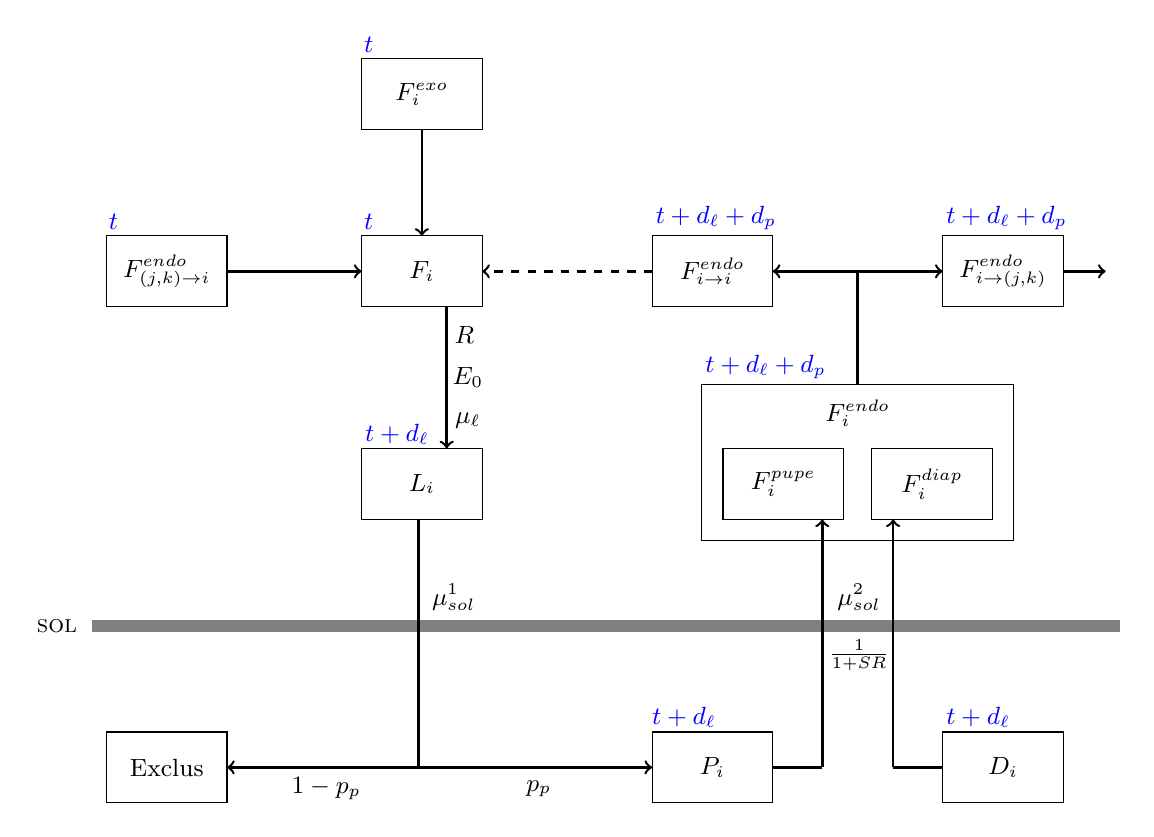
\begin{tikzpicture}[scale = 0.9]
 \draw (0, 0) node{\small \textsc{sol}};
  \draw [line width = 1.5mm, color = gray] (0.5, 0) -- (15, 0);
  % RECTANGLES
  \draw (0.7,  -1.5) rectangle (2.4,  -2.5); %diap + mort
  \draw (8.4,  -1.5) rectangle (10.1, -2.5); % P
  \draw (12.5, -1.5) rectangle (14.2, -2.5); %Diap
  \draw (4.3,   1.5) rectangle (6,   2.5); % L
  \draw (9.4,   1.5) rectangle (11.1,  2.5); % N pupe
  \draw (11.5,  1.5) rectangle (13.2,  2.5); % N diap
  \draw (9.1,   1.2) rectangle (13.5,  3.4); % N emer
  \draw (4.3,   7) rectangle (6,   8); % N exo
  \draw (0.7,   4.5) rectangle (2.4,   5.5); % N voisins
  \draw (8.4,   4.5) rectangle (10.1,  5.5); % N endo
  \draw (12.5,  4.5) rectangle (14.2,  5.5); % N degage
  \draw (4.3,   4.5) rectangle (6, 5.5); % N
  % TEXTES CASES
  \draw (1.55, -2) node {\small Exclus};
  \draw (1.55,  5) node {\small $F^\text{endo}_{(j,k) \rightarrow i}$};
  \draw (5.15,   7.5) node {\small $F^\text{exo}_{i}$};
  \draw (5.15,   2) node {\small $L_{i}$};
  \draw (5.15,   5) node {\small $F_{i}$};
  \draw (13.35, 5) node {\small $F^\text{endo}_{i\rightarrow (j,k)}$};
  \draw (9.25,  5) node {\small $F^\text{endo}_{i\rightarrow i}$};
  \draw (9.25, -2) node {\small $P_{i}$};
  \draw (13.35,-2) node {\small $D_{i}$};
  \draw (12.35, 2) node {\small $F^{\text{diap}}_{i}$};
  \draw (10.25, 2) node {\small $F^{\text{pupe}}_{i}$};
  \draw (11.3,  3) node {\small $F^{\text{endo}}_{i}$};
  \draw (0.8, 5.7) node {\small $\textcolor{blue}{t}$};
  \draw (4.4, 5.7) node {\small $\textcolor{blue}{t}$};
  \draw (4.4, 8.2) node {\small $\textcolor{blue}{t}$};
  \draw (4.8, 2.7) node {\small $\textcolor{blue}{t + d_{\ell}}$};
  \draw (8.85, -1.3) node {\small $\textcolor{blue}{t + d_{\ell}}$};
  \draw (13, -1.3) node {\small $\textcolor{blue}{t + d_{\ell}}$};
  \draw (10, 3.65) node {\small $\textcolor{blue}{t + d_{\ell} + d_{\text{p}}}$};
  \draw (9.3, 5.75) node {\small $\textcolor{blue}{t + d_{\ell} + d_{\text{p}}}$};
  \draw (13.4, 5.75) node {\small $\textcolor{blue}{t + d_{\ell} + d_{\text{p}}}$};
  % LIGNES FLECHES
  \draw [line width=0.9]     (5.1,   1.5) -- (5.1,  -2);
  \draw [->,  line width=0.9] (5.1,  -2  ) -- (2.4,  -2);
  \draw [->,  line width=0.9] (5.1,  -2  ) -- (8.4,  -2);
  \draw [line width=0.9]     (10.1, -2  ) -- (10.8, -2);
  \draw [line width=0.9]     (12.5, -2  ) -- (11.8, -2);
  \draw [->,  line width=0.9] (10.8,  -2 ) -- (10.8,  1.5);
  \draw [->,  line width=0.9] (11.8,  -2 ) -- (11.8,  1.5);
  \draw [line width=0.9]     (11.3,  3.4) -- (11.3,  5);
  \draw [->,  line width=0.9] (11.3,   5 ) -- (10.1,  5);
  \draw [->,  line width=0.9] (11.3,   5 ) -- (12.5,  5);
  \draw [->,  line width=0.9] (14.2,   5 ) -- (14.8,  5);
  \draw [->,  line width=0.9, dashed] (8.4,   5) -- (6, 5);
  \draw [->,  line width=0.9] (5.5,  4.5) -- (5.5, 2.5);
  \draw [->,  line width=0.9] (5.15,   7 ) -- (5.15,  5.5);
  \draw [->,  line width=0.9] (2.4,   5 ) -- (4.3,  5);
  % PARAMÈTRES
  \draw (5.6, 0.4)   node {\small $\mu_{\text{sol}}^1$};
  \draw (11.32, 0.4) node {\small $\mu_{\text{sol}}^2$};
  \draw (6.8, -2.3)    node {\small $p_{\text{p}}$};
  \draw (3.8, -2.3)    node {\small $1-p_{\text{p}}$};
  \draw (11.32, -0.42)  node {\small $\frac{1}{1 + SR}$};
  \draw (5.75, 4.1)     node {\small $R$};
  \draw (5.8, 3.5)     node {\small $E_0$};
  \draw (5.8, 2.9)     node {\small $\mu_\ell$};
 \end{tikzpicture}
 \caption{Schéma conceptuel du modèle pour la sous-parcelle $i$. En bleu est visible la date, la flèche en pointillés marque une rupture du temps.}
 \label{fig:schema}
\end{figure}


\section{Inflorescences}

Le modèle prendra en entrée les inflorescences.
Il faut cependant noter qu'il ne prendra pas les inflorescences «brutes», mais des dynamiques modifiées.
En effet, on émet également l'hypothèse que les cécidomyies n'attaquent non pas les toutes les inflorescences mais uniquement celles se situant au stades phénologiques C, D ou E.
Ce qui correspond aux seize premiers jours de l'inflorescence.
Pour parvenir à avoir lesdites dynamiques, on a besoin de procéder à quelques étapes intermédiaires.
On a notamment besoin de la date de débourrements des inflorescences avant d'avoir une estimation des dynamiques voulues.

\subsection{Débourrements}

 Afin de pouvoir simuler des dynamiques d'inflorescences avec une durée de vie de seize jours, il est nécessaire d'avoir les dates de débourrements des inflorescences.
 Dans le verger n\textdegree1, les dynamiques pour les modalités «enherbement ras» et «paillage synthétique» issues des deux jeux de données ont des dynamiques plutôt similaires ; on pourrait donc utiliser les débourrements du \emph{dataset 1} mis à l'échelle.
 En revanche, pour la modalité «enherbement haut», on observe des dynamiques très différentes. 
 Et comme l'on souhaite privilégier les dynamiques issues du \emph{dataset 2}, il faut procéder autrement.
 (Il en va de même pour les modalités «enherbement ras» et «paillage synthétique» du verger n\textdegree2.)
 
 L'objectif est alors de simuler les dates de débourrements qui permettent de produire la dynamique d'inflorescences vivantes du \emph{dataset 2}.
 Pour cela, on suppose que la durée de vie effective d'une inflorescence suit une loi normale.
 On possède les durées de vies effectives dans le \emph{dataset 1}.
 Premièrement, en fixant le risque de première espèce à $\alpha = 5\%$, un test de normalité de Shapiro--Wilk nous confirme la normalité ($p$-valeur de 0.05447, on ne rejette donc pas l'hypothèse de normalité).
 Deuxièmement, on observe une durée de vie effective moyenne de 29 jours (avec un écart-type de 14).
 Ainsi, il faut donc simuler des débourrements, pour que des inflorescences ayant une durée de vie qui suit une $\mathcal{N}\left( 29; 14 \right)$, donne la dynamique d'inflorescences vivantes du \emph{dataset 2}.
 Il faut donc trouver les $B_t$ tels que 
 \[
 I_{t}^{2} = B_t + \sum_{j = 1}^{50} B_{t - j} \times \left( 1 - F\left( j \right) \right),  \qquad \text{ avec } B_{t} = 0 \text{ si } t \leq 0,
 \]
 où $F$ est la fonction de répartition d'une $\mathcal{N}\left( 29;14 \right)$.
 
 Par souci d'homogénéïté, on utilisera les débourrements simulés pour les trois modalités, et ce pour les deux vergers.
 
 
\subsection{Dynamiques}


Une fois les dates de débourrements obtenus, on peut simuler des dynamiques d'inflorescences aux stades phénologiques C, D et E.
Ces inflorescences \emph{attractives} peuvent se calculer en utilisant la formule
\[
I_{t}^{a} = B_t + \sum_{t = 1}^{16} B_{t-j} \times \left( 1 - F(j) \right), \qquad \text{ avec } B_{t} = 0 \text{ si } t \leq 0. 
\]
Ici, $B_t$ représente toujours le nombre de débourrements à la date $t$ et $F$ la fonction de répartition d'une $\mathcal{N}\left( 29; 14 \right)$.
